%We showed an example of directly modelling the scheduling semantics in AGREE. But for complicated contracts (e.g. involving history), this is not a straightforward task. Thus, we model the scheduling semantics behind the scene during the AGREE translation. We propose a new AGREE usage flow, where a user has to choose the desired MoC (synchronous or scheduled AGREE) under which the contracts are to be verified. The choice of MoC is inspired by the concept of \emph{director} adopted in the Ptolemy project \cite{Ptolemy}. If the scheduled AGREE is chosen, the user also needs to specify a schedule. Currently, we assume a model of the schedule in AGREE is provided. Then, the AGREE translator will generate the corresponding Lustre model reflecting the desired semantics. 

AGREE uses a dialect \cite{GAO2008111} of the Lustre language as its backend. The AADL models with AGREE contracts are first translated to a Lustre model. The Lustre dialect introduced an expression called \emph{condact}, which is similar to the activation condition in SCADE.
It clocks a node as follows: 
\begin{equation*}
condact (cond, node(node\_inputs, node\_outputs), init\_outputs)
\end{equation*}
If the Boolean signal $cond$ is true, node $node$ is activated and updates its local and output signals. Otherwise, the node keeps the previous value of the local and output signals. Before the first activation, the node outputs values are set to \emph{init\_outputs}. %\emph{condact} is essential to model the scheduling semantics. 
We are aware that the standard Lustre language introduced similar temporal operators like \emph{when} and \emph{current}. We use \emph{condact} simply because it is supported by the underlying SMT solver.

In AGREE, each AADL thread is translated to a Lustre node, where the thread input and output ports are both mapped to the node input signals. Thus, the \emph{condact} expression does not automatically freeze the thread outputs. We add assertions to enforce the output freeze rule. And we use the thread \emph{complete} signal to clock the node. Figure \ref{WPMlustre} shows one example. 

\begin{figure}[ht!]
\centering
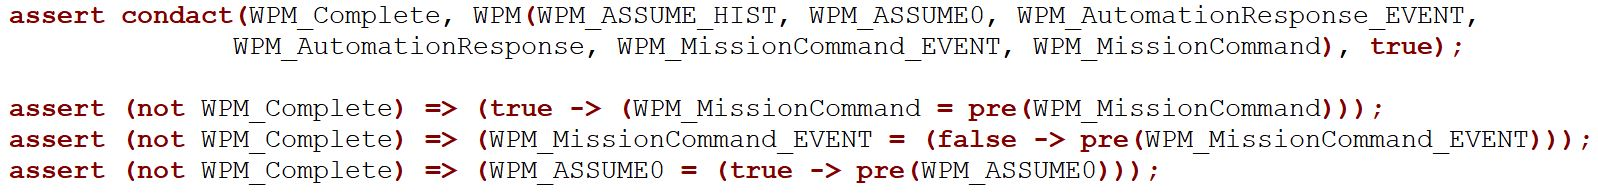
\includegraphics[width=120mm]{lustreAsync5.jpg}
\caption{A Lustre Model of a Scheduled AADL Thread \label{WPMlustre}}
\end{figure}

%\begin{figure}[ht!]
%\centering
%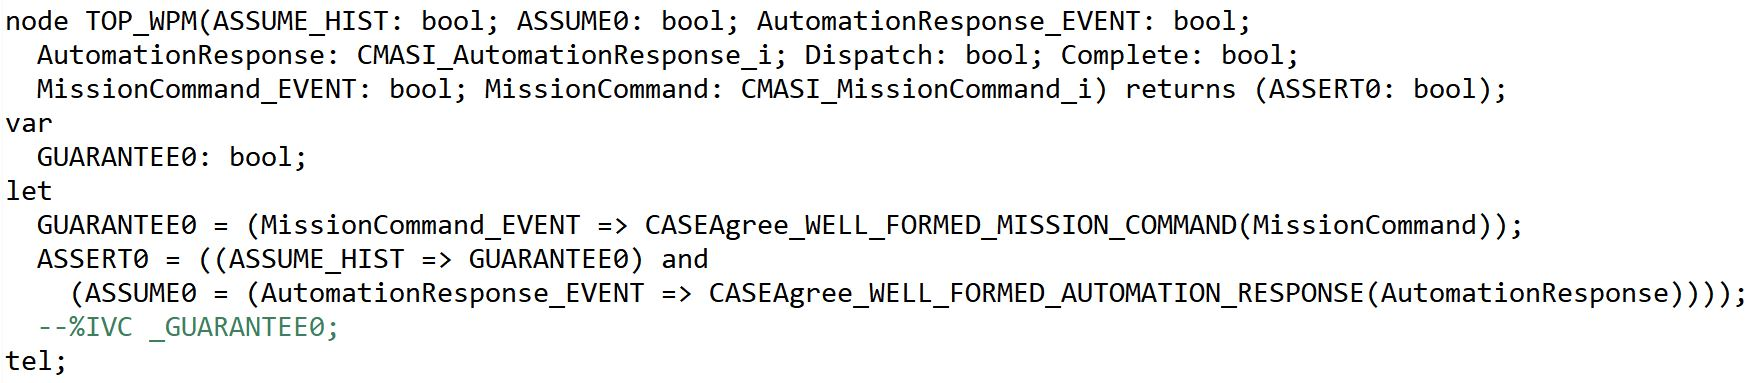
\includegraphics[width=130mm]{wpmLustre2.jpg}
%\caption{A Lustre Model of AADL Thread \label{WPMlustre}}
%\end{figure}
%
%\begin{figure}[ht!]
%\centering
%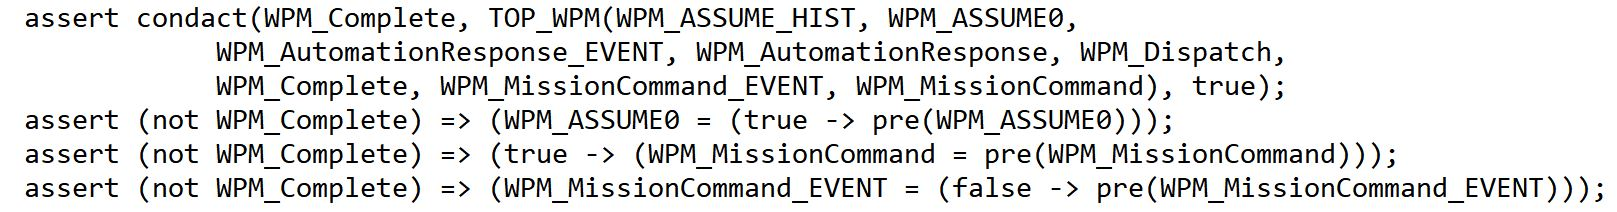
\includegraphics[width=130mm]{lustreAsync4.jpg}
%\caption{A Lustre Expression \emph{condact} Usage Example\label{lustreAsync}}
%\end{figure}
%
%\begin{figure}[ht!]
%\centering
%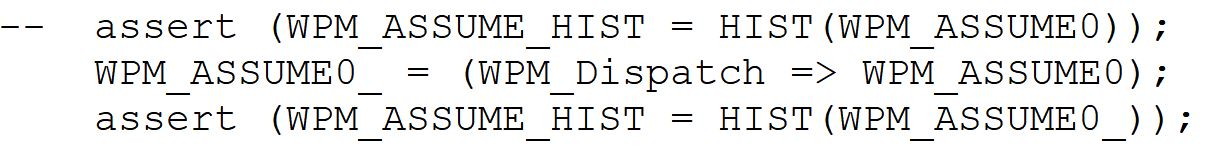
\includegraphics[width=80mm]{LustreAssume.jpg}
%\caption{An Example of Assumption Model in Lustre \label{lustreAsync}}
%\end{figure}

%\begin{figure}[ht!]
%\centering
%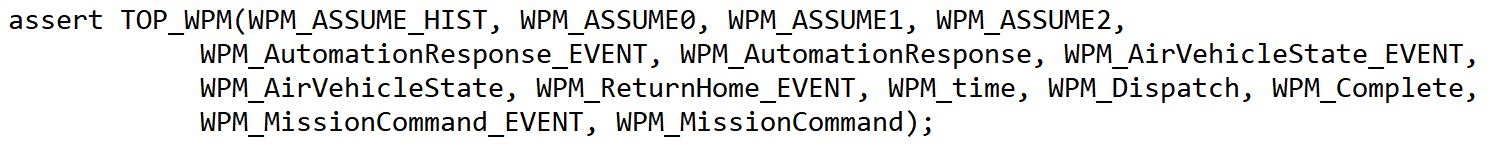
\includegraphics[width=120mm]{lustreSync2.jpg}
%\caption{An AADL Model Illustrating Motivation\label{lustreSync}}
%\end{figure}

%\begin{lstlisting}[language=c,frame=single,caption=An AGREE model of a schedule,label=schedule_model]
%  assert condact(WPM__Complete, _TOP__WPM(WPM____ASSUME__HIST, WPM____ASSUME0, WPM____ASSUME1, WPM____ASSUME2, 
%				WPM__AutomationResponse___EVENT_, WPM__AutomationResponse, WPM__AirVehicleState___EVENT_, WPM__AirVehicleState, 
%                WPM__ReturnHome___EVENT_, WPM__time, WPM__Dispatch, WPM__Complete, WPM__MissionCommand___EVENT_, WPM__MissionCommand), true);
%  assert (not WPM__Complete) => (WPM____ASSUME0 = (true -> pre(WPM____ASSUME0)));
%  assert (not WPM__Complete) => (WPM____ASSUME1 = (true -> pre(WPM____ASSUME1)));
%  assert (not WPM__Complete) => (WPM____ASSUME2 = (true -> pre(WPM____ASSUME2)));
%  assert (not WPM__Complete) => (true -> (WPM__MissionCommand = pre(WPM__MissionCommand)));
%  assert (not WPM__Complete) => (WPM__MissionCommand___EVENT_ = (false -> pre(WPM__MissionCommand___EVENT_)));
%\end{lstlisting}  
  